J'ai effectué cette seconde année d'alternance dans le centre de service (CDS) Distribution/Transporteur dédiée à la SNCF et regroupant plus de 130 collaborateurs. Il est divisé en deux périmètres distincts, mais qui peuvent tout de même être amené à travailler ensemble sur certains projets. Le premier, Transporteur, gère les applications à destination du personnel roulant de la SNCF (contrôleurs par exemple), la traçabilité de la qualité de service et les différents référentiels du système d'information (taxations, plan de transport, client...). Je travaille dans le second, Distribution.

\clearpage
\subsection{Périmètre Distribution}

    Ce périmètre prend en charge les applications concernant la vente de billet de train et leur gestion (après vente, espace client, tarification...). Cela va de la borne automatique à l'application de vente dédiée aux vendeurs en gare ou en ligne directe.
    
    \begin{figure}[!h]
        \centering
            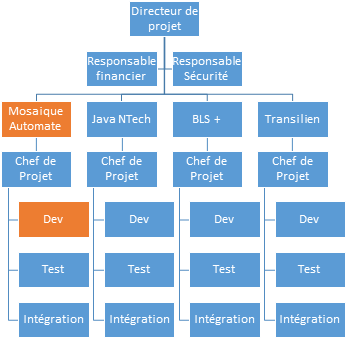
\includegraphics[width=10cm]{img/organigrameDistrib.png}
            \caption{Organigramme du périmètre Distribution}
            \label{fig:orgDistrib}
    \end{figure}

    Je suis affecté au pôle Mosaique - Automate, plus précisément dans l'équipe Dev. Ce pôle gère différentes applications :
    
    \begin{itemize}
        \item Alert Express : Permet d'afficher des alertes en temps réel sur le postes de vente Mosaique.
        \item Mosaique : Application de vente de billet de train à destination des vendeurs, que ce soit au gichet, au téléphonne en ligne directe, ou en agence pour des ventes de groupe et bien d'autre. Cette application est très importante par sa taille comme par son nombre fonctionalité primordiale pour la SNCF. Elle offre une interface graphique permettant de vendre presque tous les billets de train possibles. C'est principalement sur cette application que je travail.
        \item Olaf : Application de gestion des carte famille nombreuse. C'est en effet à la SNCF de gérer ce programme sociale de réduction.
        \item Pandore : Gestion sécurisé des transaction bancaires.
        \item RefParc3 : Gestion du matériel utilisé pour la vente sur les différent site de la SNCF sur la France entière. j'ai très récément été affecté à ce projet de taille plus modeste en parallèle de Mosaique
        \item Service Edition Billet : Gestion des envoie de mails pour la vente de billet électronique.
        \item Yield : Application de régulation du prix des billet en fonction de la demande et des places disponible. C'est cette application qui définit les prix et leur variations. 
    \end{itemize}